% Project report in IEEE conference format (IEEEtran, Times, two columns).
% Compile with pdfLaTeX (e.g. Overleaf: New Project > Upload > Recompile).
% Self-contained: every diagram and chart is drawn with TikZ/pgfplots; no image files.
% Every number comes from reports/*.json|md in the repository (regenerated 14 Nov 2026).
\documentclass[conference,a4paper]{IEEEtran}
\usepackage[T1]{fontenc}
\usepackage[utf8]{inputenc}
\usepackage{amsmath}
\usepackage{newtxtext,newtxmath}  % Times, as in IEEE papers
\usepackage{microtype}
\usepackage{booktabs}
\usepackage{tabularx}
\usepackage{array}
\usepackage{xcolor}
\usepackage{graphicx}
\usepackage{enumitem}
\usepackage{tikz}
\usetikzlibrary{arrows.meta,positioning}
\usepackage{pgfplots}
\pgfplotsset{compat=1.17}
\usepackage{cite}
\usepackage[hidelinks]{hyperref}

\definecolor{accent}{HTML}{0E7490}
\definecolor{warn}{HTML}{B45309}
\definecolor{dronered}{HTML}{D6452A}
\definecolor{unkviolet}{HTML}{7A4FD6}
\definecolor{lowamber}{HTML}{D99A0B}
\definecolor{nogray}{HTML}{8A8984}
\setlist{itemsep=1pt,topsep=3pt,leftmargin=*}
\newcolumntype{L}[1]{>{\raggedright\arraybackslash}p{#1}}
\newcolumntype{Y}{>{\raggedright\arraybackslash}X}

% A boxed one-line takeaway at the end of each results subsection.
\newcommand{\takeaway}[1]{\par\smallskip\noindent\fcolorbox{accent}{accent!6}{\parbox{\dimexpr\linewidth-2\fboxsep-2\fboxrule}{\small\textbf{Takeaway.} #1}}\par\smallskip}

\title{Counter-Drone Detection from Sound and Radio: Acoustic and 2.4\,GHz RF Detection
with Uncertainty, Open-Set Flags and Late Fusion}

\author{\IEEEauthorblockN{Vidhi Rojasara (AU2644022) \qquad Kathan Desai (AU2644002)}
\IEEEauthorblockA{AI Lab, Course Instructor: Prof.\ Maitrik Shah\\
Ahmedabad University, Ahmedabad, India}}

\begin{document}
\maketitle

\begin{abstract}
We built a system that decides, for every second of sound, whether a drone is present, and that can
add evidence from the drone's 2.4\,GHz radio link. It answers with one of four states:
\emph{No Drone}, \emph{Known Drone}, \emph{Unknown Drone} or \emph{Low Confidence}. All models are
trained and tested on public datasets with strict rules that stop test data leaking into training.
Indoors the audio detector reaches PR-AUC 0.968. Outdoors, on recordings it never heard, it catches
22\% of drone windows (66 of 300) while raising false alarms on only 1\% of non-drone windows. Our
first radio model scored almost perfectly but called pure noise ``drone''; we found this shortcut and
retrained it, and the new model (v2) catches 289 of 291 test windows and 9 of 10 drones from a
receiver it never saw. Combining sound and radio helps only when the drone transmits. No public
dataset records both for the same flight, so the fusion results are an upper bound. A dashboard
shows the audio, radio and final decision side by side.
\end{abstract}

\begin{IEEEkeywords}
drone detection, audio classification, RF signal classification, uncertainty, open-set
recognition, sensor fusion
\end{IEEEkeywords}

% =====================================================================
\section{Introduction}

\subsection{The problem}
Small drones are cheap, quiet and hard to see, which makes them a risk near campuses, prisons and
events. Two clues give a drone away: the hum of its rotors and the radio link to its controller.
Both are hard to read in the real world: wind, traffic, speech, music and helicopters cover the
sound, and Wi-Fi and Bluetooth share the same radio band.

Public drone datasets often give scores close to 100\%. Many of them come from \emph{one recording
session}, so a model can learn the room, microphone or receiver instead of the drone.

\subsection{Our goal}
\begin{enumerate}
  \item Build a drone detector from sound, with radio as a research extension.
  \item Measure honestly how well it works on data it was \emph{not} trained on, including outdoors.
  \item Say when the system is unsure, instead of always answering yes or no.
\end{enumerate}

\subsection{What we built}
\begin{itemize}
  \item A leakage-safe data pipeline over 18,093 audio clips and two radio datasets.
  \item Audio models: a classical baseline, a pretrained network with a trained head (deployed),
        and CNN, CNN+GRU, CNN+LSTM and transformer models trained from scratch.
  \item Four output states built from uncertainty and ``unknown drone'' flags.
  \item Radio models (v1, and v2 after fixing a shortcut) and a test on a second receiver.
  \item Late fusion of audio and radio evidence, with a full comparison of combination rules.
  \item A dashboard and a live operations console; 182 automated tests.
\end{itemize}

\subsection{Main results at a glance}
Table~\ref{tab:glance} answers the main questions. Every later section explains one row.

\begin{table*}[!t]
\centering\small
\caption{Main results at a glance}
\label{tab:glance}
\begin{tabularx}{\textwidth}{@{}L{5.2cm} Y L{2.8cm}@{}}
\toprule
Question & Answer & Section \\
\midrule
Does audio detection work indoors? & Yes: PR-AUC 0.968; 87.8\% of drone windows caught & \ref{sec:audio-tiers} \\
On a drone model never heard? & Mostly: PR-AUC 0.929; 64.7\% caught & \ref{sec:audio-tiers} \\
Outdoors? & Weakly: 22\% of drone windows (66/300) at 1\% false alarms; 14 of 30 drone recordings alarmed & \ref{sec:audio-tiers} \\
Which audio model is best outdoors? & A small CNN trained from scratch: PR-AUC 0.831 (deployed model 0.649) & \ref{sec:models} \\
Does radio detection work? & RF v2: 289/291 drone windows, 4/390 false alarms; 9 of 10 unseen drones & \ref{sec:rf} \\
Was the first radio model honest? & No: it called 100\% of pure noise ``drone'' (fixed in v2) & \ref{sec:rf} \\
Does combining sound and radio help? & Only when the drone transmits; for a radio-silent drone the evidence sum keeps 18.4\%, a learned combiner 0.2\% & \ref{sec:fusion} \\
False alarms on real aircraft? & None on 99 aircraft and 317 outdoor-ambience recordings & \ref{sec:outdoor} \\
\bottomrule
\end{tabularx}
\end{table*}

% =====================================================================
\section{Datasets}

We used only public datasets (Table~\ref{tab:data}); nothing was recorded by us.

\begin{table*}[!t]
\centering\small
\caption{Datasets}
\label{tab:data}
\begin{tabularx}{\textwidth}{@{}L{3.2cm} L{2.8cm} Y L{3.6cm}@{}}
\toprule
Dataset & Type & Contents & Used for \\
\midrule
DroneAudioDataset~\cite{droneaudio} & Audio, indoor & Parrot Bebop and Mambo; 1,332 drone clips (from 312 recordings), about 10,370 background clips, 1\,s each & Main training data \\
ESC-50~\cite{esc50} & Audio labels & Names of background sounds (helicopter, engine, rain, \dots) & Labelling background clips \\
ITU ARIS Lab~\cite{aris} & Audio, outdoor & 4,491 drone and 1,000 background clips & Outdoor training (tier 4) \\
Svanstr\"om~\cite{svanstrom} & Audio, outdoor & 90 ten-second recordings: 30 drone, 30 helicopter, 30 background & Outdoor \textbf{test} \\
LibriSpeech, GTZAN & Audio & Real speech and real music & Noise tests \\
AeroSonicDB~\cite{aerosonic} & Audio, outdoor & Low-flying aircraft with ADS-B labels & False-alarm check \\
DroneRF~\cite{dronerf} & Radio & 227 pieces of 0.25\,s: Bebop 84, AR 81, Phantom 21, background 41; one lab, two receivers & Radio training and test \\
Tampere~\cite{tampere} & Radio & 11 drones, anechoic chamber, a different receiver (12 files) & Second-receiver test \\
\bottomrule
\end{tabularx}
\end{table*}

\textbf{A trap found first.} In the raw audio, the \emph{length} of a clip alone separated drone
from background perfectly (ROC-AUC 1.0). A model could have ``won'' by measuring length. Every clip
is therefore cut to exactly 1\,s at 16\,kHz mono before training.

% =====================================================================
\section{Method}

\subsection{System overview}
Sound and radio each have their own data, features and model (Fig.~\ref{fig:pipeline}). Their
scores meet only at the fusion step, which feeds the four output states.

\begin{figure*}[!t]
\centering
\resizebox{\textwidth}{!}{%
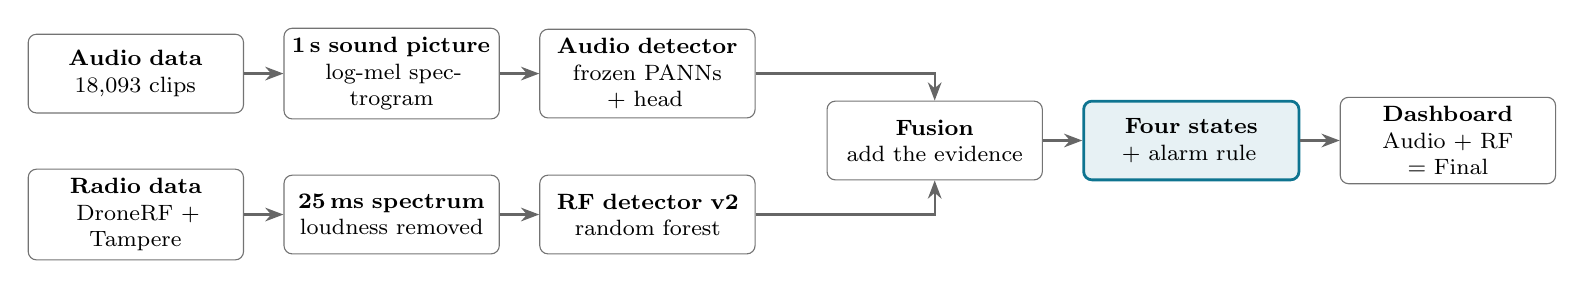
\begin{tikzpicture}[
  node distance=4mm and 5mm,
  box/.style={draw=black!55, rounded corners=3pt, align=center, font=\footnotesize,
              minimum height=10mm, text width=25mm},
  key/.style={box, draw=accent, fill=accent!10, line width=1pt},
  arr/.style={-Stealth, thick, draw=black!60}]
  \node[box] (ad) {\textbf{Audio data}\\18,093 clips};
  \node[box, right=of ad] (af) {\textbf{1\,s sound picture}\\log-mel spectrogram};
  \node[box, right=of af] (am) {\textbf{Audio detector}\\frozen PANNs + head};
  \node[box, below=7mm of ad] (rd) {\textbf{Radio data}\\DroneRF + Tampere};
  \node[box, right=of rd] (rf) {\textbf{25\,ms spectrum}\\loudness removed};
  \node[box, right=of rf] (rm) {\textbf{RF detector v2}\\random forest};
  \node[box, right=9mm of am, yshift=-8.5mm] (fu) {\textbf{Fusion}\\add the evidence};
  \node[key, right=of fu] (st) {\textbf{Four states}\\+ alarm rule};
  \node[box, right=of st] (db) {\textbf{Dashboard}\\Audio + RF = Final};
  \draw[arr] (ad) -- (af); \draw[arr] (af) -- (am);
  \draw[arr] (rd) -- (rf); \draw[arr] (rf) -- (rm);
  \draw[arr] (am) -| (fu); \draw[arr] (rm) -| (fu);
  \draw[arr] (fu) -- (st); \draw[arr] (st) -- (db);
\end{tikzpicture}%
}
\caption{System overview. In this project the radio windows come from recorded datasets; there is
no live radio receiver.}
\label{fig:pipeline}
\end{figure*}

\subsection{Audio pipeline}
\begin{enumerate}
  \item Cut the sound into 1\,s windows (a new window every 0.5\,s).
  \item Turn each window into a 64-band \textbf{log-mel spectrogram}: a picture of which pitches
        are loud at each moment.
  \item Pass it through \textbf{PANNs MobileNetV1}~\cite{panns}, a 4.2\,M-parameter network
        pretrained on AudioSet. It is \emph{frozen} (not changed) and outputs 1,024 numbers.
  \item A \textbf{logistic-regression head} turns these into a drone score from 0 to 1.
  \item Three flags are added: score near the threshold, sound unlike the training data, and
        drone-like but unlike every known drone.
\end{enumerate}
We froze the network because the data has many near-copies of few recordings; a large trainable
network would memorise them. Grad-CAM~\cite{gradcam} shows which parts of the picture pushed the
score towards ``drone''.

\subsection{Radio (RF) pipeline}
\begin{enumerate}
  \item Cut each 0.25\,s DroneRF piece into ten \textbf{25\,ms windows}.
  \item Compute a Welch \textbf{power spectrum} per window: energy at each frequency, 1,025 values
        for each half of the 2.4\,GHz band.
  \item Remove each band's average level, so loudness cannot act as a shortcut.
  \item Average into 64 sub-bands per band (128 numbers) and score with a \textbf{random forest}.
\end{enumerate}

\subsection{Four output states}
Each window gets one state (Table~\ref{tab:states}). A whole recording raises an alarm only after
\textbf{two drone windows in a row}; an isolated hit gives \emph{Low Confidence}.

\begin{table}[!t]
\centering\footnotesize
\caption{The four output states}
\label{tab:states}
\begin{tabularx}{\linewidth}{@{}L{1.9cm} Y@{}}
\toprule
State & Meaning \\
\midrule
\textcolor{nogray}{\textbf{No Drone}} & Evidence below the threshold. Not proof that no drone is present. \\
\textcolor{dronered}{\textbf{Known Drone}} & Drone-like and similar to training drones. Does not name the drone model. \\
\textcolor{unkviolet}{\textbf{Unknown Drone}} & Drone-like, but unlike every drone seen in training. \\
\textcolor{lowamber}{\textbf{Low Confidence}} & Near the threshold or unfamiliar input: a person should review. \\
\bottomrule
\end{tabularx}
\end{table}

\subsection{Fusion of audio and radio}
\begin{enumerate}
  \item Each sensor keeps its own model and score.
  \item Each score becomes \textbf{evidence}, a log-likelihood ratio (LLR), using Platt
        scaling~\cite{platt} fitted on that sensor's validation data. Positive favours ``drone'',
        0 means no information.
  \item Each LLR is capped at $\pm 5$ so one sensor cannot dominate.
  \item The two are combined, and a threshold set for 1\% false alarms decides.
\end{enumerate}
\begin{align*}
  \text{Evidence sum:}  \quad f &= \mathrm{LLR}_\text{audio} + \mathrm{LLR}_\text{RF}\\
  \text{Learned layer:} \quad f &= 1.00\,\mathrm{LLR}_\text{audio} + 1.60\,\mathrm{LLR}_\text{RF} + b
\end{align*}
A missing sensor contributes 0 and has its own threshold.

\subsection{Fair testing}
\begin{enumerate}
  \item \textbf{Split by recording.} All slices of one recording go to the same group (radio: by
        blocks of consecutive time). A checker stops the pipeline on any leak.
  \item \textbf{Three groups:} \emph{train} teaches, \emph{validation} picks settings and the
        threshold, \emph{test} is used once for the reported number.
  \item \textbf{Threshold fixed in advance:} set so 1\% of non-drone validation windows alarm.
  \item \textbf{Metrics:} PR-AUC (95\% intervals resample whole recordings), recall and
        false-alarm rate. Accuracy and F1 are not headline metrics: test sets are 12--33\% drone,
        far more than in real life.
\end{enumerate}
Table~\ref{tab:split} shows the indoor split and Table~\ref{tab:tiers} the four test tiers.
Section~\ref{sec:training} gives the training settings of every model.

\begin{table}[!t]
\centering\footnotesize
\caption{Indoor split used by all audio models}
\label{tab:split}
\begin{tabular}{@{}lrrrr@{}}
\toprule
Group & Clips & Drone & Background & Recordings \\
\midrule
Train & 8,066 & 900 & 7,166 & 1,578 \\
Validation & 1,632 & 187 & 1,445 & 336 \\
Test (tier 1) & 2,004 & 245 & 1,759 & 401 \\
\bottomrule
\end{tabular}
\end{table}

\begin{table}[!t]
\centering\footnotesize
\caption{Four test tiers, from easy to hard}
\label{tab:tiers}
\begin{tabularx}{\linewidth}{@{}l L{1.9cm} Y@{}}
\toprule
Tier & Trained on & Tested on \\
\midrule
1 & Indoor & Other indoor recordings \\
2 & Bebop only & Mambo (a drone never heard) \\
3 & Indoor & Outdoor Svanstr\"om \\
4 & Indoor + ITU ARIS & Outdoor Svanstr\"om \\
\bottomrule
\end{tabularx}
\end{table}

% =====================================================================
\section{Model Training Details}\label{sec:training}

Table~\ref{tab:train} lists every trained model and how it was trained. Table~\ref{tab:variants}
lists each training change we tried and what it did.

\begin{table*}[!t]
\centering\footnotesize
\caption{Every trained model}
\label{tab:train}
\begin{tabularx}{\textwidth}{@{}L{3.3cm} L{2.9cm} Y L{3.2cm} L{2.6cm}@{}}
\toprule
Model (script) & Input & Architecture and size & Optimisation & Epochs; selection \\
\midrule
Classical baseline (\texttt{train\_baseline.py}) & 128-band log-mel, 3 statistics per band (384 features) & Logistic regression (C\,=\,0.1); HistGradientBoosting (max depth 3) & scikit-learn & ---; threshold at 1\% val.\ FPR \\
\textbf{Pretrained head, deployed} (\texttt{train\_pretrained.py}, \texttt{train\_outdoor.py}) & 64-band log-mel & Frozen PANNs MobileNetV1 (4.2\,M) + logistic head ($\approx$1,025 weights), C\,=\,0.01, balanced classes; tier 4 also balances datasets & scikit-learn, inputs standardised on train & ---; threshold at 1\% val.\ FPR \\
Uncertainty layer (\texttt{eval\_uncertainty.py}) & Head score + embedding & Review band (10\% of val.\ windows nearest the threshold), familiarity distance, small ensemble & Fitted on validation & --- \\
Random-forest audio baseline (\texttt{train\_audio\_baseline.py}) & 64 mel means + 64 std (128) & 300 trees, balanced subsample, seed 42 & --- & ---; threshold by val.\ F1 \\
AudioCNN (\texttt{train\_audio\_cnn.py}) & 64$\times$101 log-mel & 3 conv blocks (16/32/64), global pooling, dropout 0.3 & AdamW, lr $10^{-3}$, wd $10^{-4}$, batch 128, weighted BCE, CPU & max 20, patience 4: ran 11, best 7 \\
CNN / CNN+GRU / Transformer (\texttt{train\_deep.py}) & 128$\times$63 log-mel, SpecAugment & 211k / 270k / 317k parameters & AdamW, lr $2\cdot10^{-3}$, wd $10^{-2}$, batch 128, one-cycle & 20 fixed, no early stop \\
Compact sweep (\texttt{compare\_audio\_architectures.py}) & Log-mel pooled to 64$\times$21 & Small CNN 23,585; CNN+GRU 56,129; CNN+LSTM 62,401; transformer 72,641 & Early stop on val.\ PR-AUC & ran/best 8/8, 8/6, 6/4, 8/7 \\
\midrule
RF v1: LR / forest / 1D-CNN (\texttt{train\_rf.py}) & Spectrum, 128 features & LR C\,=\,0.1; forest 300 trees; 1D-CNN 4 conv layers, $\approx$12k & CNN: Adam, lr $10^{-3}$, wd $10^{-4}$, batch 64 & CNN: 40 fixed \\
\textbf{RF v2, deployed} (\texttt{train\_rf\_v2.py}) & Same 128 features & Same forest; training data changed (Sec.~\ref{sec:rf}) & --- & ---; threshold 0.342 \\
Fusion (\texttt{eval\_fusion.py}) & Audio and RF scores & Platt calibration to LLR, cap $\pm$5; sum or learned layer & Fitted on validation pairs & --- \\
\bottomrule
\end{tabularx}
\end{table*}

\begin{table*}[!t]
\centering\footnotesize
\caption{What each training change did}
\label{tab:variants}
\begin{tabularx}{\textwidth}{@{}L{5.2cm} Y L{2.6cm}@{}}
\toprule
Change & Effect on test data & Adopted? \\
\midrule
Add outdoor ITU ARIS drones (tier 3 $\rightarrow$ 4) & Outdoor PR-AUC 0.649 $\rightarrow$ 0.640 (no gain); false alarms 19/600 $\rightarrow$ 6/600 & Yes (deployed) \\
Frozen pretrained head $\rightarrow$ CNN from scratch & Outdoor PR-AUC 0.649 $\rightarrow$ 0.831; drone vs helicopter 0.58 $\rightarrow$ 0.91 & Next step \\
Random-forest baseline $\rightarrow$ AudioCNN (tier 1) & PR-AUC 0.954 $\rightarrow$ 0.989; recall 0.886 $\rightarrow$ 0.959; F1 0.904 $\rightarrow$ 0.933 & Experiment \\
Noise augmentation (one noisy copy per clip) & 0\,dB recall: real speech 0.269 $\rightarrow$ 0.584, real music 0.449 $\rightarrow$ 0.559; clean unchanged & Experiment \\
Svanstr\"om helicopter/background negatives & PR-AUC 0.867 $\rightarrow$ 0.948; recall 0.250 $\rightarrow$ 0.213; helicopter false alarms 2/60 $\rightarrow$ 0/60 & Experiment \\
Music mixtures & Drones caught under loud music 17\% $\rightarrow$ 45\% & Experiment \\
Speaker-to-microphone copies & Played-back drones 45\% $\rightarrow$ 61\%; worse on clean audio & Opt-in only \\
Outdoor aircraft negatives & No improvement & No \\
RF v1 $\rightarrow$ v2 (new training data) & Pure noise called drone 1.000 $\rightarrow$ 0.080; unseen drones 0.954 recall & Yes (deployed) \\
RF v2 $\rightarrow$ v2b (+ band-level feature) & Did not fix Phantom; noise false alarms 0.100 & No \\
Evidence sum $\rightarrow$ learned fusion layer & Radio-silent drone recall 0.184 $\rightarrow$ 0.002 & No (sum kept) \\
\bottomrule
\end{tabularx}
\end{table*}

% =====================================================================
\section{Results}

\subsection{Audio across the four tiers}\label{sec:audio-tiers}

\begin{table}[!t]
\centering\footnotesize
\caption{Deployed audio model by tier}
\label{tab:audio}
\begin{tabular}{@{}lccc@{}}
\toprule
Tier & PR-AUC & Recall & False alarms \\
\midrule
1 Indoor & 0.968 & 0.878 & 10/1,759 \\
2 New drone & 0.929 & 0.647 & 22/2,113 \\
3 Outdoor & 0.649 & 0.330 & 19/600 \\
4 Outdoor + training & 0.640 & 0.220 & 6/600 \\
\bottomrule
\end{tabular}
\end{table}

Table~\ref{tab:audio} shows a large drop from indoor to outdoor. For tier 4 the PR-AUC 95\% interval
is 0.503--0.755. Per whole recording, 14 of 30 drone, 1 of 30 helicopter and 0 of 30 background
recordings raised an alarm. The classical baseline scores 0.981, 0.891, 0.702 and 0.619 PR-AUC on
tiers 1--4. The main confusion is helicopters: drone-vs-helicopter ROC-AUC is about 0.58.

\takeaway{Strong indoors and on a new drone model; weak outdoors.}

\subsection{Comparing audio models}\label{sec:models}

\begin{table}[!t]
\centering\footnotesize
\setlength{\tabcolsep}{3pt}
\caption{PR-AUC of each audio model by tier}
\label{tab:models}
\begin{tabular}{@{}lccccc@{}}
\toprule
Tier & CNN & CNN+GRU & Transf. & Deployed & Baseline \\
\midrule
1 & 0.986 & 0.979 & 0.985 & 0.968 & 0.981 \\
2 & 0.919 & 0.817 & 0.926 & 0.929 & 0.891 \\
3 & \textbf{0.831} & 0.810 & 0.702 & 0.649 & 0.702 \\
4 & \textbf{0.796} & 0.791 & 0.673 & 0.640 & 0.619 \\
\midrule
Drone vs heli. & \textbf{0.911} & 0.898 & 0.799 & $\approx$0.58 & $\approx$0.74 \\
\bottomrule
\end{tabular}
\end{table}

The small CNN trained from scratch is the best outdoor model and separates helicopters far better
(Table~\ref{tab:models}). The transformer is best on the unseen drone (tier-2 recall 0.716) but
weakest outdoors. The GRU adds nothing over the CNN: 1\,s windows hold little temporal structure.
In the compact sweep, CNN+GRU leads indoors (0.985) and the compact CNN outdoors (0.814); recurrent
and transformer models have outdoor recall of only 0.12--0.14.

\takeaway{Switching to the from-scratch CNN is the clearest next improvement.}

\subsection{Robustness to noise}
Tier-1 test clips were mixed with unseen noise at 20, 10 and 0\,dB, with the threshold fixed.
At 20\,dB recall changes by at most 0.016. Fig.~\ref{fig:noise} shows 0\,dB, where the noise is as
loud as the drone.

\begin{figure}[!t]
\centering
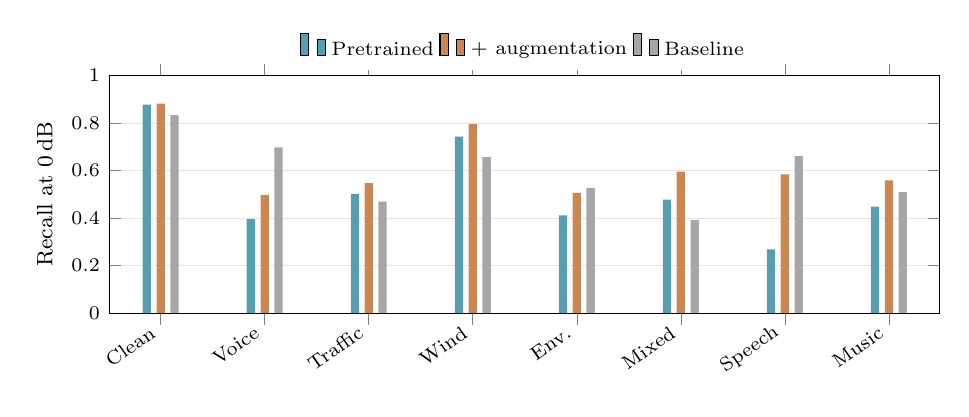
\begin{tikzpicture}
\begin{axis}[
  ybar, bar width=3pt, width=\linewidth, height=4.6cm,
  ymin=0, ymax=1, ylabel={Recall at 0\,dB}, ylabel style={font=\footnotesize},
  symbolic x coords={Clean,Voice,Traffic,Wind,Env.,Mixed,Speech,Music},
  xtick=data, x tick label style={rotate=35, anchor=east, font=\scriptsize},
  y tick label style={font=\scriptsize},
  legend style={at={(0.5,1.02)}, anchor=south, legend columns=3, font=\scriptsize, draw=none},
  ymajorgrids, grid style={black!10}, enlarge x limits=0.07]
\addplot[fill=accent!70, draw=none] coordinates {(Clean,0.878) (Voice,0.396) (Traffic,0.502) (Wind,0.743) (Env.,0.412) (Mixed,0.478) (Speech,0.269) (Music,0.449)};
\addplot[fill=warn!70, draw=none] coordinates {(Clean,0.882) (Voice,0.498) (Traffic,0.547) (Wind,0.796) (Env.,0.506) (Mixed,0.596) (Speech,0.584) (Music,0.559)};
\addplot[fill=black!35, draw=none] coordinates {(Clean,0.833) (Voice,0.698) (Traffic,0.469) (Wind,0.657) (Env.,0.527) (Mixed,0.392) (Speech,0.661) (Music,0.510)};
\legend{Pretrained, + augmentation, Baseline}
\end{axis}
\end{tikzpicture}
\caption{Recall at 0\,dB SNR. ``Speech'' and ``Music'' are real recordings (LibriSpeech, GTZAN).}
\label{fig:noise}
\end{figure}

Augmentation improves every condition, including real speech (+0.31) and music (+0.11) it never
trained on. Loud music is the only noise causing many false alarms (7--9\% at 0\,dB).

\takeaway{Noise augmentation helps everywhere; loud music remains the main threat.}

\subsection{Uncertainty and unknown drones}

\begin{table}[!t]
\centering\footnotesize
\setlength{\tabcolsep}{3pt}
\caption{Low Confidence flag by tier}
\label{tab:unc}
\begin{tabular}{@{}lcccc@{}}
\toprule
Tier & Error rate & Flagged & Error if not flagged & Errors caught \\
\midrule
1 & 0.020 & 12.7\% & 0.005 & 80\% \\
3 & 0.244 & 41.8\% & 0.218 & 48\% \\
4 & 0.267 & 11.6\% & 0.245 & 19\% \\
\bottomrule
\end{tabular}
\end{table}

The Low Confidence flag catches most mistakes indoors but few outdoors (Table~\ref{tab:unc}). Trained
on Bebop only, the Unknown Drone flag separates the unseen Mambo at AUROC 0.81.

\takeaway{The flags work indoors; they do not yet detect the move outdoors.}

\subsection{Radio: a shortcut found and fixed}\label{sec:rf}

\textbf{RF v1} (trained on DroneRF only) reached PR-AUC 1.000, even on drones left out of training.
Two checks showed this was false:
\begin{enumerate}
  \item On windows with \emph{no visible signal}, it still separated drone sessions from background
        sessions (AUC 1.000).
  \item On the Tampere recordings from another receiver, it called \textbf{100\% of pure noise}
        ``drone'' (median score 0.88).
\end{enumerate}
It had learned the \emph{recording session}, not the drone. \textbf{RF v2} keeps the same model and
changes only the training data: silent windows from drone sessions are no longer labelled drone,
simulated receiver noise is added as ``not drone'', and Tampere drones from a second receiver are
added, split by drone. Table~\ref{tab:rf} compares the two.

\begin{table}[!t]
\centering\footnotesize
\setlength{\tabcolsep}{3pt}
\caption{Radio model v1 vs v2}
\label{tab:rf}
\begin{tabularx}{\linewidth}{@{}Y cc@{}}
\toprule
Check & v1 & v2 \\
\midrule
Pure noise called drone (worst type) & 1.000 & \textbf{0.080} \\
Tampere white-noise check & 1.000 & \textbf{0.000} \\
Silent drone-session windows called drone & all & \textbf{0.000} \\
Unseen Tampere drones, mean recall & --- & \textbf{0.954} \\
Test: drones caught / false alarms & --- & 289/291, 4/390 \\
Left-out DroneRF Phantom recall & 0.976 & 0.024 \\
\bottomrule
\end{tabularx}
\end{table}

v2 catches 9 of 10 unseen Tampere drones at recall 1.000 (Parrot Mambo 0.542). It misses a
left-out Phantom, whose video link fills the band evenly and, with loudness removed, looks like
raised noise. Temperature scaling~\cite{guo} lowers test calibration error from 0.0166 to 0.0069;
the held-out Phantom is flagged as unknown at ROC-AUC 0.769. Drone type is identified correctly in
291 of 320 test windows (same session).

\takeaway{v2 detects transmissions, not the session; real Wi-Fi/Bluetooth false alarms are untested.}

\subsection{Fusion of sound and radio}\label{sec:fusion}
Each test pair is an outdoor audio window and a radio window of the same class, drawn
independently: 4,000 pairs per class and scenario (Table~\ref{tab:fusion}).

\begin{table*}[!t]
\centering\small
\caption{Fusion ablation: recall / false-alarm rate}
\label{tab:fusion}
\begin{tabular}{@{}lccc@{}}
\toprule
Method & Both sensors see the drone & Drone with no radio link & Radio sees only noise \\
\midrule
Audio only & 0.225 / 0.007 & 0.223 / 0.012 & 0.224 / 0.010 \\
RF only & 0.993 / 0.000 & 0.000 / 0.000 & 0.993 / 0.013 \\
OR rule & 0.995 / 0.007 & 0.223 / 0.012 & 0.993 / 0.023 \\
AND rule & 0.224 / 0.000 & 0.000 / 0.000 & 0.224 / 0.000 \\
\textbf{Evidence sum (deployed)} & \textbf{0.995 / 0.005} & \textbf{0.184 / 0.008} & 0.992 / 0.028 \\
Learned layer & 0.996 / 0.000 & 0.002 / 0.000 & 0.995 / 0.022 \\
\bottomrule
\end{tabular}
\end{table*}

\begin{itemize}
  \item With both sensors, fusion equals RF alone ($\approx$99\%). RF's test negatives come from one
        lab, so this is RF's best case.
  \item For a \textbf{radio-silent drone}, the evidence sum keeps most of audio's recall (0.184 vs
        0.223); the learned layer falls to 0.002, because it never saw a drone without radio while
        learning. We therefore deploy the sum. This choice was made after seeing these test
        results.
  \item Helicopter false alarms fall from 0.014 (audio only) to 0.011 (sum).
\end{itemize}

\takeaway{Use the evidence sum. All fusion numbers are an upper bound: sound and radio were never
recorded together.}

\subsection{Outdoor checks}\label{sec:outdoor}
\begin{itemize}
  \item \textbf{Real aircraft} (AeroSonicDB, held-out sessions): no alarm on any of 99 aircraft or
        317 outdoor-ambience recordings, partly because the detector is cautious outdoors.
  \item \textbf{Live alarm rule}, set on validation recordings: alarms on 57\% of outdoor drone test
        recordings and on 1.7\% of background recordings.
\end{itemize}

% =====================================================================
\section{Implementation}

\subsection{Software}
\begin{itemize}
  \item \texttt{src/dronedet}: data, splits, features, models, evaluation, fusion, four-state rules,
        media decoding.
  \item \texttt{scripts/}: 30+ scripts; each regenerates one report in \texttt{reports/}.
  \item \texttt{tests/}: 182 automated tests (leakage, splits, features, models, four-state logic,
        media decoding, dashboard rendering).
  \item Operations console (\texttt{python -m console}): live microphone or file, incident queue,
        operator labels, retraining that is adopted only if it does better on held-out data.
\end{itemize}

\subsection{Dashboard}
Started with \texttt{streamlit run app/dashboard.py}; dark theme by default.
\begin{itemize}
  \item \textbf{Project briefing:} purpose, method, four states, headline results, limits, and a
        readiness table read from the files on disk.
  \item \textbf{Replay detector:} the result first, then \textbf{Audio + RF = Final} as three
        coloured tiles with score bars, a window-by-window strip, and Grad-CAM
        (Fig.~\ref{fig:final}).
  \item \textbf{Inputs:} dataset recordings, any audio or video file, a YouTube link, or the
        microphone. Only the sound is used; at most 5 minutes are analysed; nothing is retrained.
  \item \textbf{Fusion, Audio, RF tabs:} charts and tables taken directly from the reports.
\end{itemize}

\begin{figure*}[!t]
\centering
\resizebox{\textwidth}{!}{%
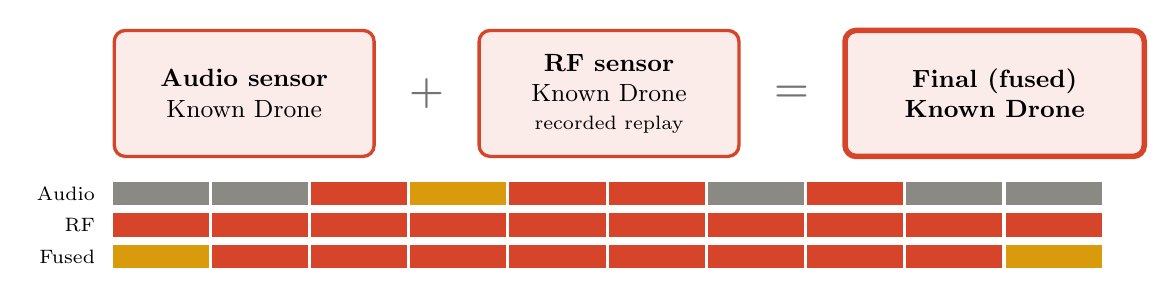
\begin{tikzpicture}[
  tile/.style={draw=#1, line width=1.2pt, rounded corners=4pt, fill=#1!10, align=center,
               font=\small, minimum width=33mm, minimum height=16mm},
  op/.style={font=\Large\bfseries, text=black!55}]
  \node[tile=dronered] (a) {\textbf{Audio sensor}\\Known Drone};
  \node[op, right=3mm of a] (p) {+};
  \node[tile=dronered, right=3mm of p] (r) {\textbf{RF sensor}\\Known Drone\\[-1pt]{\scriptsize recorded replay}};
  \node[op, right=3mm of r] (e) {=};
  \node[tile=dronered, right=3mm of e, line width=2pt, minimum width=38mm] (f) {\textbf{Final (fused)}\\\textbf{Known Drone}};
  \foreach \x/\c in {0/nogray,1/nogray,2/dronered,3/lowamber,4/dronered,5/dronered,6/nogray,7/dronered,8/nogray,9/nogray} {
    \fill[\c] ([xshift=\x*12.6mm,yshift=-6mm]a.south west) rectangle ++(12.2mm,3mm); }
  \foreach \x/\c in {0/dronered,1/dronered,2/dronered,3/dronered,4/dronered,5/dronered,6/dronered,7/dronered,8/dronered,9/dronered} {
    \fill[\c] ([xshift=\x*12.6mm,yshift=-10mm]a.south west) rectangle ++(12.2mm,3mm); }
  \foreach \x/\c in {0/lowamber,1/dronered,2/dronered,3/dronered,4/dronered,5/dronered,6/dronered,7/dronered,8/dronered,9/lowamber} {
    \fill[\c] ([xshift=\x*12.6mm,yshift=-14mm]a.south west) rectangle ++(12.2mm,3mm); }
  \node[anchor=east, font=\scriptsize] at ([xshift=-1mm,yshift=-4.5mm]a.south west) {Audio};
  \node[anchor=east, font=\scriptsize] at ([xshift=-1mm,yshift=-8.5mm]a.south west) {RF};
  \node[anchor=east, font=\scriptsize] at ([xshift=-1mm,yshift=-12.5mm]a.south west) {Fused};
\end{tikzpicture}%
}
\caption{The dashboard's final-decision view (illustration). Top: each sensor's verdict and the fused
verdict. Bottom: one row per sensor over time (grey No Drone, red Known Drone, amber Low
Confidence). With radio added, the result is an unpaired what-if.}
\label{fig:final}
\end{figure*}

\subsection{Reproducibility check}
On 14 November 2026 we rebuilt all radio and fusion models on a fresh machine:
\begin{enumerate}
  \item All 23 DroneRF archives and 12 Tampere files matched their published checksums.
  \item The radio features were rebuilt: 2,270 windows, segment counts exactly as in the DroneRF
        paper (84, 81, 21, 41).
  \item RF v1, calibration, RF v2 and both fusion rules were retrained.
\end{enumerate}
RF v1 forest and logistic regression, the Tampere check and RF v2 reproduced exactly; fusion moved
by at most 0.0003. Only the small RF v1 1D-CNN changed (recall $\pm$0.01--0.04), as CPU training of
a neural network is not bit-for-bit repeatable.

% =====================================================================
\section{Discussion}

\subsection{What the results show}
\begin{itemize}
  \item Audio detection works indoors and on an unseen drone model.
  \item Outdoors it catches about one in five drone windows at 1\% false alarms.
  \item A near-perfect radio benchmark score was a session shortcut; v2 removes it.
  \item For a radio-silent drone only audio helps; the evidence sum keeps it.
\end{itemize}

\subsection{What they do not show}
\begin{itemize}
  \item Performance at a real deployment site.
  \item Fusion on sound and radio recorded together (no such public dataset exists).
  \item Radio false alarms on real Wi-Fi and Bluetooth traffic.
  \item Calibrated audio probabilities, or the drone model inside the four states.
\end{itemize}

\subsection{Limitations}
\begin{itemize}
  \item Some pretrained-head settings were chosen while looking at all tiers, including tier 3;
        those rows are mildly optimistic.
  \item Test sets are 12--33\% drone. At 1\% drone windows, tier-4 precision would fall from 0.917
        to about 0.18.
  \item Noise is added at fixed SNR: no echo, distance or microphone effects.
  \item The fusion rule was chosen after seeing test results.
\end{itemize}

% =====================================================================
\section{Conclusion and Future Work}
We built an acoustic drone detector with fair, leakage-controlled testing and four-state output,
a radio extension whose first version we proved to be a shortcut and then fixed, and an audio-radio
fusion study. Our clearest finding is a warning: benchmark scores near 1.0 did not survive a second
receiver or the move outdoors.

\textbf{Next steps:}
\begin{enumerate}
  \item Deploy the from-scratch CNN and re-fit the uncertainty flags.
  \item Record real Wi-Fi and Bluetooth radio data outside the DroneRF lab.
  \item Record sound and radio of the same flights to test fusion properly.
  \item Connect a real radio receiver (SDR) and collect field recordings.
\end{enumerate}

\begin{thebibliography}{11}
\bibitem{dronerf} M.~S. Allahham, M.~F. Al-Sa'd, A.~Al-Ali, A.~Mohamed, T.~Khattab, and A.~Erbad, ``DroneRF dataset: A dataset of drones for RF-based detection, classification and identification,'' \emph{Data in Brief}, 2019.
\bibitem{panns} Q.~Kong, Y.~Cao, T.~Iqbal, Y.~Wang, W.~Wang, and M.~D. Plumbley, ``PANNs: Large-scale pretrained audio neural networks for audio pattern recognition,'' \emph{IEEE/ACM Trans. Audio, Speech, Lang. Process.}, 2020.
\bibitem{droneaudio} S.~Al-Emadi, A.~Al-Ali, A.~Mohammad, and A.~Al-Ali, ``Audio based drone detection and identification using deep learning,'' in \emph{Proc. IWCMC}, 2019.
\bibitem{svanstrom} F.~Svanstr\"om, F.~Alonso-Fernandez, and C.~Englund, ``A dataset for multi-sensor drone detection,'' \emph{Data in Brief}, 2021.
\bibitem{esc50} K.~J. Piczak, ``ESC: Dataset for environmental sound classification,'' in \emph{Proc. ACM Multimedia}, 2015.
\bibitem{tampere} Tampere University, ``Drone RF recordings,'' Zenodo, record 4264467, CC BY 4.0.
\bibitem{aris} ITU ARIS Lab, ``Drone audio dataset,'' Zenodo, record 22682339.
\bibitem{aerosonic} ``AeroSonicDB (YPAD-0523): acoustic aircraft detection dataset.''
\bibitem{platt} J.~Platt, ``Probabilistic outputs for support vector machines and comparisons to regularized likelihood methods,'' in \emph{Advances in Large Margin Classifiers}, 1999.
\bibitem{guo} C.~Guo, G.~Pleiss, Y.~Sun, and K.~Q. Weinberger, ``On calibration of modern neural networks,'' in \emph{Proc. ICML}, 2017.
\bibitem{gradcam} R.~R. Selvaraju \emph{et al.}, ``Grad-CAM: Visual explanations from deep networks via gradient-based localization,'' in \emph{Proc. ICCV}, 2017.
\end{thebibliography}

\end{document}
